\documentclass[11pt,a4paper]{article}

\usepackage[T1]{fontenc}
\usepackage{charter}
\usepackage{microtype}
\usepackage{amsmath,amssymb}
\usepackage[a4paper,margin=20mm]{geometry}
\usepackage{xcolor}
\usepackage{booktabs}
\usepackage{tabularx}
\usepackage{listings}
\renewcommand{\lstlistingname}{Listing}
\usepackage{fancyhdr}
\usepackage{tikz}
\usetikzlibrary{arrows.meta,positioning,shapes.geometric}
\usepackage{hyperref}

\definecolor{primary}{RGB}{15,76,129}
\definecolor{codebg}{RGB}{247,249,252}
\definecolor{codeframe}{RGB}{210,220,232}
\definecolor{commentclr}{RGB}{90,105,120}
\definecolor{kwclr}{RGB}{0,82,155}
\definecolor{strclr}{RGB}{163,21,21}

\hypersetup{
    colorlinks=true,
    linkcolor=primary,
    citecolor=primary,
    urlcolor=primary,
    pdftitle={Technical Specification and Source Code Analysis: ARMv7 Embedded Linux Bring-Up and ISO C23 Telemetry Monitor},
    pdfauthor={Embedded Linux Engineering Portfolio}
}

\setlength{\parskip}{6pt plus 2pt minus 1pt}
\setlength{\parindent}{0pt}

\pagestyle{fancy}
\fancyhf{}
\fancyhead[L]{\small\color{commentclr}Embedded Linux Portfolio --- Project 02 (ARMv7 Cortex-A9 / ISO C23)}
\fancyhead[R]{\small\color{commentclr}Engineering Specification for Dev Team}
\fancyfoot[C]{\small\thepage}
\renewcommand{\headrulewidth}{0.4pt}

\lstdefinestyle{cstyle}{
    backgroundcolor=\color{codebg},
    frame=single,
    rulecolor=\color{codeframe},
    basicstyle=\ttfamily\footnotesize,
    keywordstyle=\color{kwclr}\bfseries,
    commentstyle=\color{commentclr}\itshape,
    stringstyle=\color{strclr},
    breaklines=true,
    breakatwhitespace=true,
    showstringspaces=false,
    numbers=left,
    numberstyle=\tiny\color{commentclr},
    numbersep=6pt,
    tabsize=4,
    captionpos=b
}
\lstset{style=cstyle}

\newcommand{\takeaway}[2]{%
  \vspace{6pt}\noindent\colorbox{primary!8}{%
    \parbox{\dimexpr\linewidth-2\fboxsep\relax}{%
      \vspace{4pt}\textbf{\color{primary}#1:}\hspace{0.5em}#2\vspace{4pt}%
    }%
  }\vspace{6pt}%
}

\title{\vspace{-1.2cm}\textbf{\color{primary}Technical Specification, System Architecture, and Exhaustive Source Code Analysis:\\
ARMv7 Embedded Linux Bring-Up from Scratch and ISO C23 Telemetry Monitor}}
\author{Engineering Documentation Prepared for Peer Development Review}
\date{November 2026}

\begin{document}
\maketitle
\thispagestyle{empty}

\begin{abstract}
This technical specification documents, justifies, and audits the complete ISO/IEC 9899:2024 (C23) source code and build-automation pipeline of \textbf{Project 2: ARMv7 Embedded Linux Bring-Up \& C23 Telemetry Monitor}. Unlike turnkey environments built around pre-packaged vendor Board Support Packages (BSPs), this architecture constructs all four foundational layers of an Embedded Linux system from upstream sources on the emulated \emph{ARM Versatile Express Cortex-A9} (\texttt{vexpress-a9}) platform in QEMU: the cross-compilation toolchain (\texttt{arm-linux-gnueabihf}), bootloader (\emph{Das U-Boot v2025.10}), kernel (\emph{Linux Kernel 6.12 LTS}) with out-of-tree \emph{Device Tree}, and minimal root filesystem (\emph{BusyBox 1.37.0} in \emph{Initramfs}) hosting the deterministic telemetry monitor \texttt{sysmon\_c23}. Every design choice, defensive macro, integer-overflow guard, and build patch is grounded in authoritative systems engineering literature, safety-critical coding standards (\emph{MISRA C:2025}, \emph{CERT C}), and official upstream documentation.
\end{abstract}

\tableofcontents
\newpage

% ==============================================================================
\section{Global System Architecture and Boot Model}
% ==============================================================================

A production Embedded Linux system requires tight, deterministic integration across four independent software layers: the cross-compilation toolchain, the bootloader, the Linux kernel with its hardware-description \emph{Device Tree Blob} (DTB), and the root filesystem (\emph{RootFS}) \cite{simmonds2017,billoo2022}. Rather than delegating this integration to a meta-build framework such as Yocto or Buildroot in this foundational project, every stage is constructed explicitly to expose the hardware-software contracts across ARMv7-A privilege levels.

\begin{figure}[!htbp]
\centering
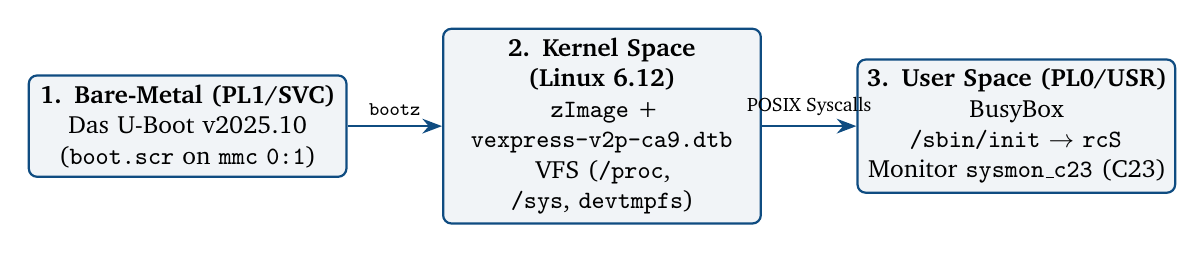
\begin{tikzpicture}[
    node distance=1.1cm and 1.2cm,
    box/.style={rectangle, draw=primary, thick, fill=primary!6, rounded corners=3pt, text width=3.8cm, align=center, minimum height=1.2cm, font=\small},
    arrow/.style={-{Stealth[length=2.5mm]}, thick, draw=primary}
]
\node[box] (uboot) {\textbf{1. Bare-Metal (PL1/SVC)}\\Das U-Boot v2025.10\\(\texttt{boot.scr} on \texttt{mmc 0:1})};
\node[box, right=of uboot] (kernel) {\textbf{2. Kernel Space (Linux 6.12)}\\ \texttt{zImage} + \texttt{vexpress-v2p-ca9.dtb}\\VFS (\texttt{/proc}, \texttt{/sys}, \texttt{devtmpfs})};
\node[box, right=of kernel] (user) {\textbf{3. User Space (PL0/USR)}\\BusyBox \texttt{/sbin/init} $\rightarrow$ \texttt{rcS}\\Monitor \texttt{sysmon\_c23} (C23)};

\draw[arrow] (uboot) -- node[above, font=\scriptsize] {\texttt{bootz}} (kernel);
\draw[arrow] (kernel) -- node[above, font=\scriptsize] {POSIX Syscalls} (user);
\end{tikzpicture}
\caption{Multi-stage execution pipeline from bare-metal U-Boot initialization to ARMv7 user-space telemetry.}
\label{fig:boot_pipeline}
\end{figure}

On the \texttt{vexpress-a9} board, physical DDR2 memory (\emph{DRAM Bank 0}) starts at address \texttt{0x60000000} \cite{qemu_vexpress}. Payload staging addresses must provide sufficient separation so that kernel self-decompression of \texttt{zImage} never overwrites the DTB or the initial RAM disk during the ARMv7 boot protocol. Table~\ref{tab:dram_map} details the deterministic DRAM layout enforced by this project.

\begin{table}[!htbp]
\centering
\caption{Physical DRAM memory map for \texttt{vexpress-a9} U-Boot hand-off.}
\label{tab:dram_map}
\begin{tabularx}{\linewidth}{l l l X}
\toprule
\textbf{Payload} & \textbf{U-Boot Variable} & \textbf{Physical Address} & \textbf{Purpose and Engineering Rationale} \\
\midrule
Boot script & *(Scratch Load)* & \texttt{0x60000000} & \texttt{boot.scr} ($\approx 300$ bytes); staged at DRAM base for \texttt{source} execution prior to kernel loading. \\
Compressed kernel & \texttt{\$\{kernel\_addr\_r\}} & \texttt{0x60100000} & \texttt{zImage}; leaves a $1\text{ MiB}$ gap above \texttt{0x60000000} and ample headroom for decompression before reaching the DTB. \\
Device Tree Blob & \texttt{\$\{fdt\_addr\_r\}} & \texttt{0x62000000} & \texttt{vexpress-v2p-ca9.dtb}; isolated $31\text{ MiB}$ above the kernel entry address to prevent decompression overlap. \\
Initial Ramdisk & \texttt{\$\{ramdisk\_addr\_r\}} & \texttt{0x63000000} & \texttt{uInitramfs}; \texttt{cpio.gz} archive wrapped with a U-Boot \texttt{mkimage} header, staged $16\text{ MiB}$ above the DTB. \\
\bottomrule
\end{tabularx}
\end{table}

% ==============================================================================
\section{ISO C23 Engineering Foundations and Safety Standards}
% ==============================================================================

The user-space telemetry monitor \texttt{sysmon\_c23} adheres to four complementary engineering standards designed to eliminate undefined behavior (UB) and guarantee deterministic execution:

\begin{enumerate}
\item \textbf{ISO/IEC 9899:2024 (C23 Standard):} Leverages the standardized \texttt{<stdckdint.h>} header for checked integer arithmetic (\texttt{ckd\_add}, \texttt{ckd\_sub}, \texttt{ckd\_mul}) \cite{gustedt2025,cppref_c23,cppref_numeric}, the type-safe \texttt{nullptr} constant (eliminating ambiguity with integer \texttt{0}), typed enumeration constants, and the \texttt{[[nodiscard]]} attribute to prevent callers from silently ignoring error codes \cite{gustedt2025}.
\item \textbf{Secure Coding (\emph{Effective C} and CERT C):} All external inputs (CLI arguments and \texttt{/proc} pseudo-files) are validated via \texttt{strtoul} with \texttt{endptr} inspection and explicit range bounds, fixed-size buffer reads via \texttt{fgets}, and deterministic \texttt{FILE *} descriptor closure along every exit path \cite{seacord2020}.
\item \textbf{Defensive Programming (\emph{Learn C the Hard Way}):} Implements a diagnostic macro layer in \texttt{dbg.h} built around the single-exit cleanup pattern (\texttt{goto error;}), refactored to comply strictly with \texttt{-std=c23 -pedantic -Werror} without relying on non-standard GNU variadic extensions \cite{shaw2015}.
\item \textbf{Safety-Critical Systems (\emph{MISRA C:2025}):} The continuous sampling loop performs \textbf{zero dynamic heap allocation} (all structs reside deterministically on the stack, preventing fragmentation and leaks), computes CPU and memory percentages in fixed-point \emph{permille} ($1/1000$) arithmetic, and compiles cleanly under \texttt{-Wconversion -Wsign-conversion} \cite{misra2025}.
\end{enumerate}

% ==============================================================================
\section{Exhaustive C Source Code Analysis (\texttt{user/sysmon\_c23/})}
% ==============================================================================

\subsection{C23 Portability Layer: \texttt{c23\_compat.h}}

Because host development environments (such as Debian 12 with GCC 12) often coexist with newer cross-compilation toolchains (GCC 14/15/16 supporting \texttt{-std=c23} \cite{gcc_dialect}), \texttt{c23\_compat.h} abstracts modern C23 primitives cleanly without altering application logic.

\begin{lstlisting}[language=C,caption={Complete source of \texttt{user/sysmon\_c23/c23\_compat.h}.}]
#ifndef SYSMON_C23_COMPAT_H
#define SYSMON_C23_COMPAT_H

#include <stdbool.h>
#include <stddef.h>
#include <stdint.h>

#if defined(__has_include) && __has_include(<stdckdint.h>)
#  include <stdckdint.h>
#else
#  define ckd_add(r, a, b) __builtin_add_overflow((a), (b), (r))
#  define ckd_sub(r, a, b) __builtin_sub_overflow((a), (b), (r))
#  define ckd_mul(r, a, b) __builtin_mul_overflow((a), (b), (r))
#endif

#if !defined(__cplusplus) && (__STDC_VERSION__ < 202311L)
#  ifndef nullptr
#    define nullptr ((void *)0)
#  endif
#  ifndef constexpr
#    define constexpr static const
#  endif
#endif

#if defined(__STDC_VERSION__) && (__STDC_VERSION__ >= 202311L)
#  define SYSMON_NODISCARD [[nodiscard]]
#elif defined(__GNUC__) || defined(__clang__)
#  define SYSMON_NODISCARD __attribute__((warn_unused_result))
#else
#  define SYSMON_NODISCARD
#endif

#endif /* SYSMON_C23_COMPAT_H */
\end{lstlisting}

\textbf{Line-by-line engineering breakdown:}
\begin{itemize}
\item \textbf{Include Guards (\texttt{\#ifndef SYSMON\_C23\_COMPAT\_H}):} Prevents multiple inclusion within a translation unit, avoiding duplicate symbol or macro redefinition errors.
\item \textbf{Compile-time \texttt{<stdckdint.h>} probing via \texttt{\_\_has\_include}:} Standardized in C23, \texttt{\_\_has\_include} inspects whether the C library provides \texttt{<stdckdint.h>}. On GCC $\ge 14$, it includes the standard header natively; on older hosts, it maps \texttt{ckd\_add}, \texttt{ckd\_sub}, and \texttt{ckd\_mul} to GCC's hardware-backed \texttt{\_\_builtin\_*\_overflow} intrinsics, which return \texttt{true} whenever the exact mathematical result exceeds the destination type's representable range \cite{cppref_numeric}.
\item \textbf{Version Macro \texttt{\_\_STDC\_VERSION\_\_ < 202311L}:} The integer constant \texttt{202311L} formally identifies ISO C23. Under \texttt{-std=c2x} on legacy compilers, \texttt{nullptr} and \texttt{constexpr} are provided as safe fallbacks; under C23, native keywords take precedence.
\item \textbf{\texttt{SYSMON\_NODISCARD} Contract:} Expands to standard \texttt{[[nodiscard]]} in C23 or \texttt{\_\_attribute\_\_((warn\_unused\_result))} in prior modes. Combined with \texttt{-Werror}, discarding any API return status becomes a hard compilation error \cite{gustedt2025}.
\end{itemize}

\subsection{Defensive Error-Handling Macros: \texttt{dbg.h}}

\texttt{dbg.h} adapts Zed Shaw's defensive logging macros \cite{shaw2015} to eliminate the non-standard GNU \texttt{\#\#\_\_VA\_ARGS\_\_} extension, which triggers diagnostics under strict \texttt{-std=c23 -pedantic -Werror} when variadic macros are invoked with zero trailing arguments.

\begin{lstlisting}[language=C,caption={Complete source of \texttt{user/sysmon\_c23/dbg.h}.}]
#ifndef SYSMON_DBG_H
#define SYSMON_DBG_H

#include <stdio.h>
#include <errno.h>
#include <string.h>

#define clean_errno() (errno == 0 ? "None" : strerror(errno))

#define log_err_msg(M) fprintf(stderr, "[ERROR] (%s:%d: errno: %s) %s\n", \
        __FILE__, __LINE__, clean_errno(), (M))

#define log_err_fmt(M, ...) fprintf(stderr, "[ERROR] (%s:%d: errno: %s) " M "\n", \
        __FILE__, __LINE__, clean_errno(), __VA_ARGS__)

#define log_info_fmt(M, ...) fprintf(stdout, "[INFO]  " M "\n", __VA_ARGS__)

#define check_msg(A, M) if (!(A)) { \
    log_err_msg(M); errno = 0; goto error; }

#define check_fmt(A, M, ...) if (!(A)) { \
    log_err_fmt(M, __VA_ARGS__); errno = 0; goto error; }

#define sentinel_msg(M) { \
    log_err_msg(M); errno = 0; goto error; }

#define sentinel_fmt(M, ...) { \
    log_err_fmt(M, __VA_ARGS__); errno = 0; goto error; }

#endif /* SYSMON_DBG_H */
\end{lstlisting}

\textbf{Technical rationale:}
\begin{itemize}
\item \textbf{\texttt{\_msg} vs \texttt{\_fmt} Separation:} In \texttt{log\_err\_msg(M)}, the message \texttt{M} is passed via \texttt{"\%s"}, which simultaneously satisfies ISO C99/C23 variadic rules and prevents format-string vulnerabilities audited by \texttt{-Wformat=2} \cite{seacord2020}. In \texttt{log\_err\_fmt(M, ...)}, at least one format argument is always supplied.
\item \textbf{Single-Exit Cleanup Pattern:} Both \texttt{check\_*} and \texttt{sentinel\_*} log the source file (\texttt{\_\_FILE\_\_}), line number (\texttt{\_\_LINE\_\_}), and human-readable \texttt{errno} string via \texttt{clean\_errno()}, reset \texttt{errno = 0}, and branch to a single local \texttt{error:} label where open \texttt{FILE *} descriptors are deterministically closed before returning \cite{shaw2015}.
\end{itemize}

\subsection{Data Structures and API Contracts: \texttt{sysmon.h}}

\begin{lstlisting}[language=C,caption={Complete source of \texttt{user/sysmon\_c23/sysmon.h}.}]
#ifndef SYSMON_H
#define SYSMON_H

#include "c23_compat.h"

enum {
    SYSMON_MAX_LINE_LEN  = 256U,
    SYSMON_MAX_MODEL_LEN = 64U
};

typedef enum {
    SYSMON_OK              =  0,
    SYSMON_ERR_NULL_PTR    = -1,
    SYSMON_ERR_IO          = -2,
    SYSMON_ERR_PARSE       = -3,
    SYSMON_ERR_OVERFLOW    = -4
} sysmon_status_t;

typedef struct {
    uint64_t user;
    uint64_t nice;
    uint64_t system;
    uint64_t idle;
    uint64_t iowait;
    uint64_t irq;
    uint64_t softirq;
    uint64_t steal;
} cpu_ticks_t;

typedef struct {
    uint64_t mem_total_kb;
    uint64_t mem_free_kb;
    uint64_t mem_available_kb;
    uint64_t buffers_kb;
    uint64_t cached_kb;
    uint64_t mem_used_kb;
    uint32_t mem_usage_permille;
} mem_stats_t;

typedef struct {
    double   uptime_sec;
    double   idle_sec;
    uint32_t load_1m_permille;
    uint32_t load_5m_permille;
    uint32_t load_15m_permille;
    char     board_model[SYSMON_MAX_MODEL_LEN];
} sys_overview_t;

SYSMON_NODISCARD sysmon_status_t sysmon_read_cpu_ticks(const char *proc_stat_path,
                                                       cpu_ticks_t *out_ticks);
SYSMON_NODISCARD sysmon_status_t sysmon_calc_cpu_usage_permille(const cpu_ticks_t *prev,
                                                                const cpu_ticks_t *curr,
                                                                uint32_t *out_permille);
SYSMON_NODISCARD sysmon_status_t sysmon_read_meminfo(const char *proc_meminfo_path,
                                                     mem_stats_t *out_mem);
SYSMON_NODISCARD sysmon_status_t sysmon_read_overview(const char *proc_uptime_path,
                                                      const char *proc_loadavg_path,
                                                      const char *dt_model_path,
                                                      sys_overview_t *out_overview);
#endif /* SYSMON_H */
\end{lstlisting}

\textbf{Design highlights:}
\begin{itemize}
\item \textbf{Enumeration Constants over Preprocessor Macros:} \texttt{SYSMON\_MAX\_LINE\_LEN} and \texttt{SYSMON\_MAX\_MODEL\_LEN} are typed integer constants, enabling fixed-size stack arrays (\texttt{char board\_model[SYSMON\_MAX\_MODEL\_LEN]}) without Variable-Length Arrays (VLAs) \cite{misra2025}.
\item \textbf{Exact-Width Types (\texttt{<stdint.h>}):} All CPU jiffies and memory counters use \texttt{uint64\_t}, preventing 32-bit wrap-around on ARMv7 targets where \texttt{unsigned long} is limited to 32 bits.
\item \textbf{Path Dependency Injection:} Every API function accepts \texttt{const char *} filesystem paths instead of hardcoding \texttt{"/proc/stat"}, enabling deterministic unit testing against mock fixtures.
\end{itemize}

\subsection{Telemetry Monitor Implementation: \texttt{sysmon\_c23.c}}

\subsubsection{Checked CPU Tick Accumulation and Mathematical Model}

The kernel pseudo-file \texttt{/proc/stat} exports cumulative scheduler tick counters in \texttt{USER\_HZ} (\emph{jiffies}) since boot \cite{man_proc_stat,love2010}. At sampling instant $k$, let the tick vector be:
\[
\mathbf{t}_k = (t_{\text{user}}, t_{\text{nice}}, t_{\text{sys}}, t_{\text{idle}}, t_{\text{iowait}}, t_{\text{irq}}, t_{\text{softirq}}, t_{\text{steal}})
\]
Total cumulative ticks are $T_k = \sum_{i=1}^{8} t_{k,i}$ and cumulative idle ticks are $I_k = t_{\text{idle}} + t_{\text{iowait}}$. Between consecutive samples $k-1$ and $k$, the deltas are $\Delta T = T_k - T_{k-1}$ and $\Delta I = I_k - I_{k-1}$. To avoid unnecessary floating-point arithmetic in embedded loops, CPU utilization in \emph{permille} (where $425 \equiv 42.5\%$) is computed as:
\begin{equation}
\text{CPU}_{\text{\textperthousand}} = \left\lfloor \frac{(\Delta T - \Delta I) \cdot 1000}{\Delta T} \right\rfloor, \quad \text{subject to } \Delta T > 0 \;\land\; \Delta I < \Delta T
\end{equation}

Inside \texttt{sum\_cpu\_ticks\_safe} and \texttt{sysmon\_calc\_cpu\_usage\_permille}, every addition, subtraction, and multiplication by \texttt{1000ULL} is guarded by \texttt{ckd\_add}, \texttt{ckd\_sub}, and \texttt{ckd\_mul}. Any counter wrap-around or 64-bit overflow immediately returns \texttt{SYSMON\_ERR\_OVERFLOW} rather than silently emitting corrupted telemetry \cite{seacord2020,cppref_numeric}.

\begin{lstlisting}[language=C,caption={Signal handler and overflow-checked CPU tick summation in \texttt{sysmon\_c23.c}.}]
static volatile sig_atomic_t g_keep_running = 1;

static void handle_signal(int sig)
{
    (void)sig;
    g_keep_running = 0;
}

SYSMON_NODISCARD static sysmon_status_t sum_cpu_ticks_safe(const cpu_ticks_t *ticks,
                                                           uint64_t *out_total,
                                                           uint64_t *out_idle_all)
{
    check_msg(ticks != nullptr && out_total != nullptr && out_idle_all != nullptr,
              "Null pointer in sum_cpu_ticks_safe");

    uint64_t total = 0U;
    uint64_t idle_all = 0U;

    if (ckd_add(&idle_all, ticks->idle, ticks->iowait)) {
        sentinel_msg("Overflow summing idle + iowait ticks");
    }

    const uint64_t fields[8] = {
        ticks->user, ticks->nice, ticks->system, ticks->idle,
        ticks->iowait, ticks->irq, ticks->softirq, ticks->steal
    };

    for (size_t i = 0U; i < 8U; ++i) {
        if (ckd_add(&total, total, fields[i])) {
            sentinel_msg("Overflow accumulating total CPU ticks");
        }
    }

    *out_total = total;
    *out_idle_all = idle_all;
    return SYSMON_OK;

error:
    return SYSMON_ERR_OVERFLOW;
}
\end{lstlisting}

\textbf{Key implementation details:}
\begin{itemize}
\item \textbf{Async-Signal Safety (\texttt{volatile sig\_atomic\_t}):} POSIX and ISO C guarantee atomic read/write access to \texttt{sig\_atomic\_t} across asynchronous signal interrupts (\texttt{SIGINT}, \texttt{SIGTERM}), while \texttt{volatile} prevents the \texttt{-O2} optimizer from caching \texttt{g\_keep\_running} in a CPU register \cite{man_sigaction,seacord2020}.
\item \textbf{Bounded Parsing of \texttt{/proc/stat} and \texttt{/proc/meminfo}:} \texttt{sysmon\_read\_cpu\_ticks} restricts line reads via \texttt{fgets} to \texttt{SYSMON\_MAX\_LINE\_LEN} bytes, eliminating stack buffer-overflow risks. \texttt{sscanf} uses portable \texttt{SCNu64} specifiers from \texttt{<inttypes.h>} and validates \texttt{matched >= 4} \cite{man_proc}. In \texttt{sysmon\_read\_meminfo}, if \texttt{MemAvailable} is absent on older kernels, the fallback sums \texttt{MemFree + Buffers + Cached}.
\item \textbf{Device Tree Model Extraction:} \texttt{sysmon\_read\_overview} reads \texttt{/proc/device-tree/model} with \texttt{fread} bounded to \texttt{sizeof(ov.board\_model) - 1U}, explicitly appends \texttt{'\textbackslash 0'}, strips trailing newlines, and falls back to \texttt{"Generic Embedded Linux Target"} on non-DT platforms.
\item \textbf{CLI Validation and POSIX Timers:} Defining \texttt{\#define \_POSIX\_C\_SOURCE 200809L} exposes \texttt{struct sigaction} and \texttt{nanosleep} \cite{man_sigaction}. CLI parameters (\texttt{iterations} and \texttt{interval\_ms}) are parsed via \texttt{strtoul} (never \texttt{atoi}, which lacks error detection \cite{seacord2020}), verifying \texttt{endptr != argv[i]}, \texttt{*endptr == '\textbackslash 0'}, and operational bounds (\texttt{1..10000} samples, \texttt{50..60000} ms).
\end{itemize}

\subsection{Application Build System: \texttt{user/sysmon\_c23/Makefile}}

\begin{itemize}
\item \textbf{Standard Auto-Detection (\texttt{CSTD\_FLAG}):} Probes whether \texttt{\$(CC)} supports \texttt{-std=c23}; if unavailable (GCC 12/13), automatically falls back to \texttt{-std=c2x} \cite{gcc_dialect}.
\item \textbf{Compiler Hardening (\texttt{CFLAGS}):} Enables \texttt{-O2 -Wall -Wextra -Werror -pedantic} alongside \texttt{-Wformat=2}, \texttt{-Wconversion -Wsign-conversion}, \texttt{-Wnull-dereference}, \texttt{-Wshadow}, \texttt{-fstack-protector-strong}, and \texttt{-D\_FORTIFY\_SOURCE=2} \cite{seacord2020}.
\item \textbf{Sanitizer Gate (\texttt{sanitize}):} Compiles and executes on the host with \texttt{-fsanitize=address,undefined -fno-omit-frame-pointer} to catch out-of-bounds accesses or UB prior to ARM cross-compilation.
\item \textbf{RootFS Deployment (\texttt{install-rootfs}):} Links statically (\texttt{-static}), strips debug symbols (\texttt{\$(STRIP)}), and installs the binary into \texttt{rootfs/usr/bin/sysmon\_c23} with mode \texttt{0755}, avoiding shared-library (\texttt{ld-linux-armhf.so}) dependencies inside the minimal \emph{Initramfs}.
\end{itemize}

% ==============================================================================
\section{Build Automation and Emulation Pipeline (\texttt{Makefile} and \texttt{scripts/})}
% ==============================================================================

All automation scripts enforce \texttt{set -euo pipefail}: \texttt{-e} aborts on non-zero exit codes, \texttt{-u} rejects uninitialized variables, and \texttt{-o pipefail} propagates failures across shell pipelines.

\subsection{Root Orchestration \texttt{Makefile}}
Coordinates idempotent stage targets: \texttt{make demo} chains \texttt{deps $\rightarrow$ build $\rightarrow$ run}; \texttt{make direct} executes \texttt{deps $\rightarrow$ build $\rightarrow$ run-direct} (4-core SMP direct kernel boot); \texttt{make clean} removes compiled app binaries and disk images; and \texttt{make distclean} purges all downloaded upstream trees (\texttt{sources/}, \texttt{Bootloader/}, \texttt{kernel/}, \texttt{rootfs/}).

\subsection{\texttt{scripts/01\_install\_deps.sh}}
Installs the ARM cross-compiler (\texttt{gcc-arm-linux-gnueabihf}), QEMU emulator (\texttt{qemu-system-arm}), kernel build dependencies (\texttt{bc}, \texttt{bison}, \texttt{flex}, \texttt{libssl-dev}, \texttt{dwarves}), disk-packaging tools (\texttt{u-boot-tools}, \texttt{cpio}, \texttt{dosfstools}, \texttt{mtools}, \texttt{fdisk}), and verification tools (\texttt{valgrind}, \texttt{cppcheck}, \texttt{gdb-multiarch}).

\subsection{\texttt{scripts/02\_build\_uboot.sh}}
Clones \emph{Das U-Boot} (\texttt{v2025.10}) with \texttt{--depth=1} and compiles out-of-tree (\texttt{O="\$\{PROJ\_ROOT\}/Bootloader"}) from \texttt{vexpress\_ca9x4\_defconfig} \cite{uboot_release}. Via \texttt{./scripts/config}, it applies two critical modifications:
\begin{enumerate}
\item Moves environment storage from NOR Flash (\texttt{CONFIG\_ENV\_IS\_IN\_FLASH}) to FAT (\texttt{CONFIG\_ENV\_IS\_IN\_FAT}) on \texttt{mmc 0:1} (\texttt{uboot.env}).
\item Enables \texttt{CONFIG\_USE\_BOOTCOMMAND=y} and sets \texttt{CONFIG\_BOOTCOMMAND="fatload mmc 0:1 0x60000000 boot.scr; source 0x60000000"}. This fixes an upstream failure in \texttt{vexpress\_ca9x4}'s default \texttt{distro\_bootcmd}, where an unset \texttt{\$\{scriptaddr\}} causes \texttt{load} to print usage help and \texttt{source} to abort at \texttt{0x90000000}.
\end{enumerate}

\subsection{\texttt{scripts/03\_build\_kernel.sh}}
Clones \emph{Linux 6.12 LTS} (\texttt{v6.12.111}) \cite{kernel_releases}, generates \texttt{vexpress\_defconfig}, enables \texttt{CONFIG\_BLK\_DEV\_INITRD}, \texttt{CONFIG\_RD\_GZIP}, \texttt{CONFIG\_DEVTMPFS\_MOUNT}, \texttt{CONFIG\_PROC\_FS}, and \texttt{CONFIG\_SYSFS}, compiles \texttt{zImage} and \texttt{dtbs}, and handles the Linux $\ge 6.5$ 32-bit ARM Device Tree directory reorganization by staging \texttt{arch/arm/boot/dts/arm/vexpress-v2p-ca9.dtb}.

\subsection{\texttt{scripts/04\_build\_busybox.sh}}
Builds \emph{BusyBox 1.37.0} \cite{busybox_site} with \texttt{CONFIG\_STATIC=y}. It patches \texttt{.config} to disable \texttt{CONFIG\_TC} (which fails against Linux $\ge 6.8$ \texttt{net/if\_packet.h} headers) and disables \texttt{CONFIG\_SHA1\_HWACCEL} and \texttt{CONFIG\_SHA256\_HWACCEL} to resolve the upstream BusyBox 1.37.0 ARM cross-compilation bug (\texttt{sha1\_process\_block64\_shaNI undeclared}) \cite{busybox_shani}. It then stages FHS directories, \texttt{/etc/inittab} (attaching the shell to \texttt{ttyAMA0}), and \texttt{/etc/init.d/rcS}.

\subsection{\texttt{scripts/05\_build\_sysmon.sh}}
Acts as an automated quality gate: runs \texttt{make sanitize} (ASan + UBSan) on the host first, and only proceeds to cross-compile the static ARMv7 binary (\texttt{make install-rootfs}) if all runtime sanitizer checks pass.

\subsection{\texttt{scripts/06\_package\_images.sh}}
Packages all boot media without requiring \texttt{sudo}:
\begin{enumerate}
\item Prepends \texttt{/usr/sbin:/sbin} to \texttt{PATH} so unprivileged Debian/Ubuntu users can invoke \texttt{mkfs.vfat} and \texttt{sfdisk}.
\item Generates \texttt{initramfs.cpio.gz} using \texttt{cpio --null -ov --format=newc --owner=+0:+0}, setting \texttt{root:root} (\texttt{0:0}) ownership without \texttt{sudo} or \texttt{fakeroot}, and wraps it with \texttt{mkimage -T ramdisk} into \texttt{uInitramfs}.
\item Compiles \texttt{boot.cmd} into \texttt{boot.scr} (\texttt{mkimage -T script}).
\item Formats a $63\text{ MiB}$ FAT32 partition (\texttt{part.img}), copies all four boot files via \texttt{mcopy} (\emph{mtools}), prepends a $1\text{ MiB}$ ($2048$-sector) MBR header into \texttt{sdcard.img}, and writes a bootable DOS partition table (\texttt{printf "label: dos\textbackslash n2048,,c,*\textbackslash n" | sfdisk sdcard.img}) so U-Boot detects \texttt{mmc 0:1} cleanly.
\end{enumerate}

\subsection{\texttt{scripts/07\_run\_qemu.sh}}
Launches \texttt{qemu-system-arm} for \texttt{-machine vexpress-a9} with $512\text{ MiB}$ RAM, multiplexed serial console (\texttt{-nographic -serial mon:stdio}), and \texttt{-audiodev none,id=noaudio} to silence PipeWire/PulseAudio warnings from the emulated ARM PL041 audio controller \cite{qemu_vexpress}:
\begin{itemize}
\item \textbf{\texttt{uboot} mode (\texttt{make demo}):} Boots \texttt{u-boot} single-core with \texttt{-drive if=sd,format=raw,file=...}. Omitting \texttt{-smp 4} prevents QEMU from releasing all four Cortex-A9 cores at address \texttt{0x0} simultaneously, which would corrupt U-Boot's bare-metal stack.
\item \textbf{\texttt{direct} mode (\texttt{make direct}):} Boots \texttt{zImage}, \texttt{vexpress-v2p-ca9.dtb}, and \texttt{initramfs.cpio.gz} directly with \texttt{-smp 4}, as QEMU's internal Linux loader parks secondary cores in \texttt{WFI} until brought online by the kernel.
\end{itemize}

% ==============================================================================
\begin{thebibliography}{99}

\bibitem{gustedt2025}
J.~Gustedt, \emph{Modern C}, 3rd~ed.\ (ISO/IEC 9899:2024 / C23).\ Manning Publications, 2025.

\bibitem{seacord2020}
R.~C.~Seacord, \emph{Effective C: An Introduction to Professional C Programming}, 2nd~ed.\ No Starch Press, 2024.

\bibitem{shaw2015}
Z.~A.~Shaw, \emph{Learn C the Hard Way: Practical Exercises on the Computational Subjects You Keep Avoiding}.\ Addison-Wesley, 2015.

\bibitem{misra2025}
MISRA Consortium, \emph{MISRA C:2025 --- Guidelines for the Use of the C Language in Critical Systems}.\ The MISRA Consortium Limited, 2025.

\bibitem{simmonds2017}
C.~Simmonds, \emph{Mastering Embedded Linux Programming}, 2nd~ed.\ Packt Publishing, 2017.

\bibitem{billoo2022}
M.~Billoo, \emph{Embedded Linux Essentials Handbook: Build Embedded Linux Systems and Real-World Apps with Yocto, Buildroot, and RPi}.\ 2022.

\bibitem{love2010}
R.~Love, \emph{Linux Kernel Development}, 3rd~ed.\ Addison-Wesley Professional, 2010.

\bibitem{cppref_c23}
cppreference, ``C23 Standard Features and Library Headers,'' 2025. [Online]. Available: \url{https://cppreference.net/c/23.html}

\bibitem{cppref_numeric}
cppreference, ``Checked Integer Arithmetic (\texttt{<stdckdint.h>}),'' 2025. [Online]. Available: \url{https://cppreference.net/c/numeric.html}

\bibitem{gcc_dialect}
Free Software Foundation, ``Options Controlling C Dialect (\texttt{-std=c23}),'' \emph{GCC Online Documentation}. [Online]. Available: \url{https://gcc.gnu.org/onlinedocs/gcc/C-Dialect-Options.html}

\bibitem{man_proc}
M.~Kerrisk, ``\texttt{proc(5)} --- Process Information Pseudo-Filesystem,'' \emph{Linux Programmer's Manual}, 2026. [Online]. Available: \url{https://man7.org/linux/man-pages/man5/proc.5.html}

\bibitem{man_proc_stat}
M.~Kerrisk, ``\texttt{proc\_stat(5)} --- Kernel and System Statistics,'' \emph{Linux Programmer's Manual}, 2026. [Online]. Available: \url{https://man7.org/linux/man-pages/man5/proc_stat.5.html}

\bibitem{man_sigaction}
M.~Kerrisk, ``\texttt{sigaction(2)} --- Examine and Change a Signal Action,'' \emph{Linux Programmer's Manual}, 2026. [Online]. Available: \url{https://man7.org/linux/man-pages/man2/sigaction.2.html}

\bibitem{qemu_vexpress}
QEMU Project, ``Arm Versatile Express Boards (\texttt{vexpress-a9}, \texttt{vexpress-a15}),'' \emph{QEMU System Emulator Documentation}. [Online]. Available: \url{https://qemu-project.gitlab.io/qemu/system/arm/vexpress.html}

\bibitem{kernel_releases}
The Linux Kernel Archives, ``Active Kernel Releases (6.12 LTS / 6.18 LTS).'' [Online]. Available: \url{https://www.kernel.org/releases.html}

\bibitem{uboot_release}
Das U-Boot Project, ``U-Boot Release Cycle and Configuration Documentation.'' [Online]. Available: \url{https://docs.u-boot.org/en/v2025.07/develop/release_cycle.html}

\bibitem{busybox_site}
BusyBox Project, ``BusyBox: The Swiss Army Knife of Embedded Linux.'' [Online]. Available: \url{https://busybox.net/}

\bibitem{busybox_shani}
BusyBox Issue Tracker, ``ARM Cross-Compilation Failure: \texttt{sha1\_process\_block64\_shaNI} Undeclared in 1.37.0.'' [Online]. Available: \url{https://github.com/mirror/busybox/issues/104}

\end{thebibliography}

\end{document}
